\section{Threat Actors}
Wichtigste Threat Actors: \textbf{Script Kiddies, Cyber-Kriminelle, APTs}
\begin{center}
    \vspace{-8pt}
    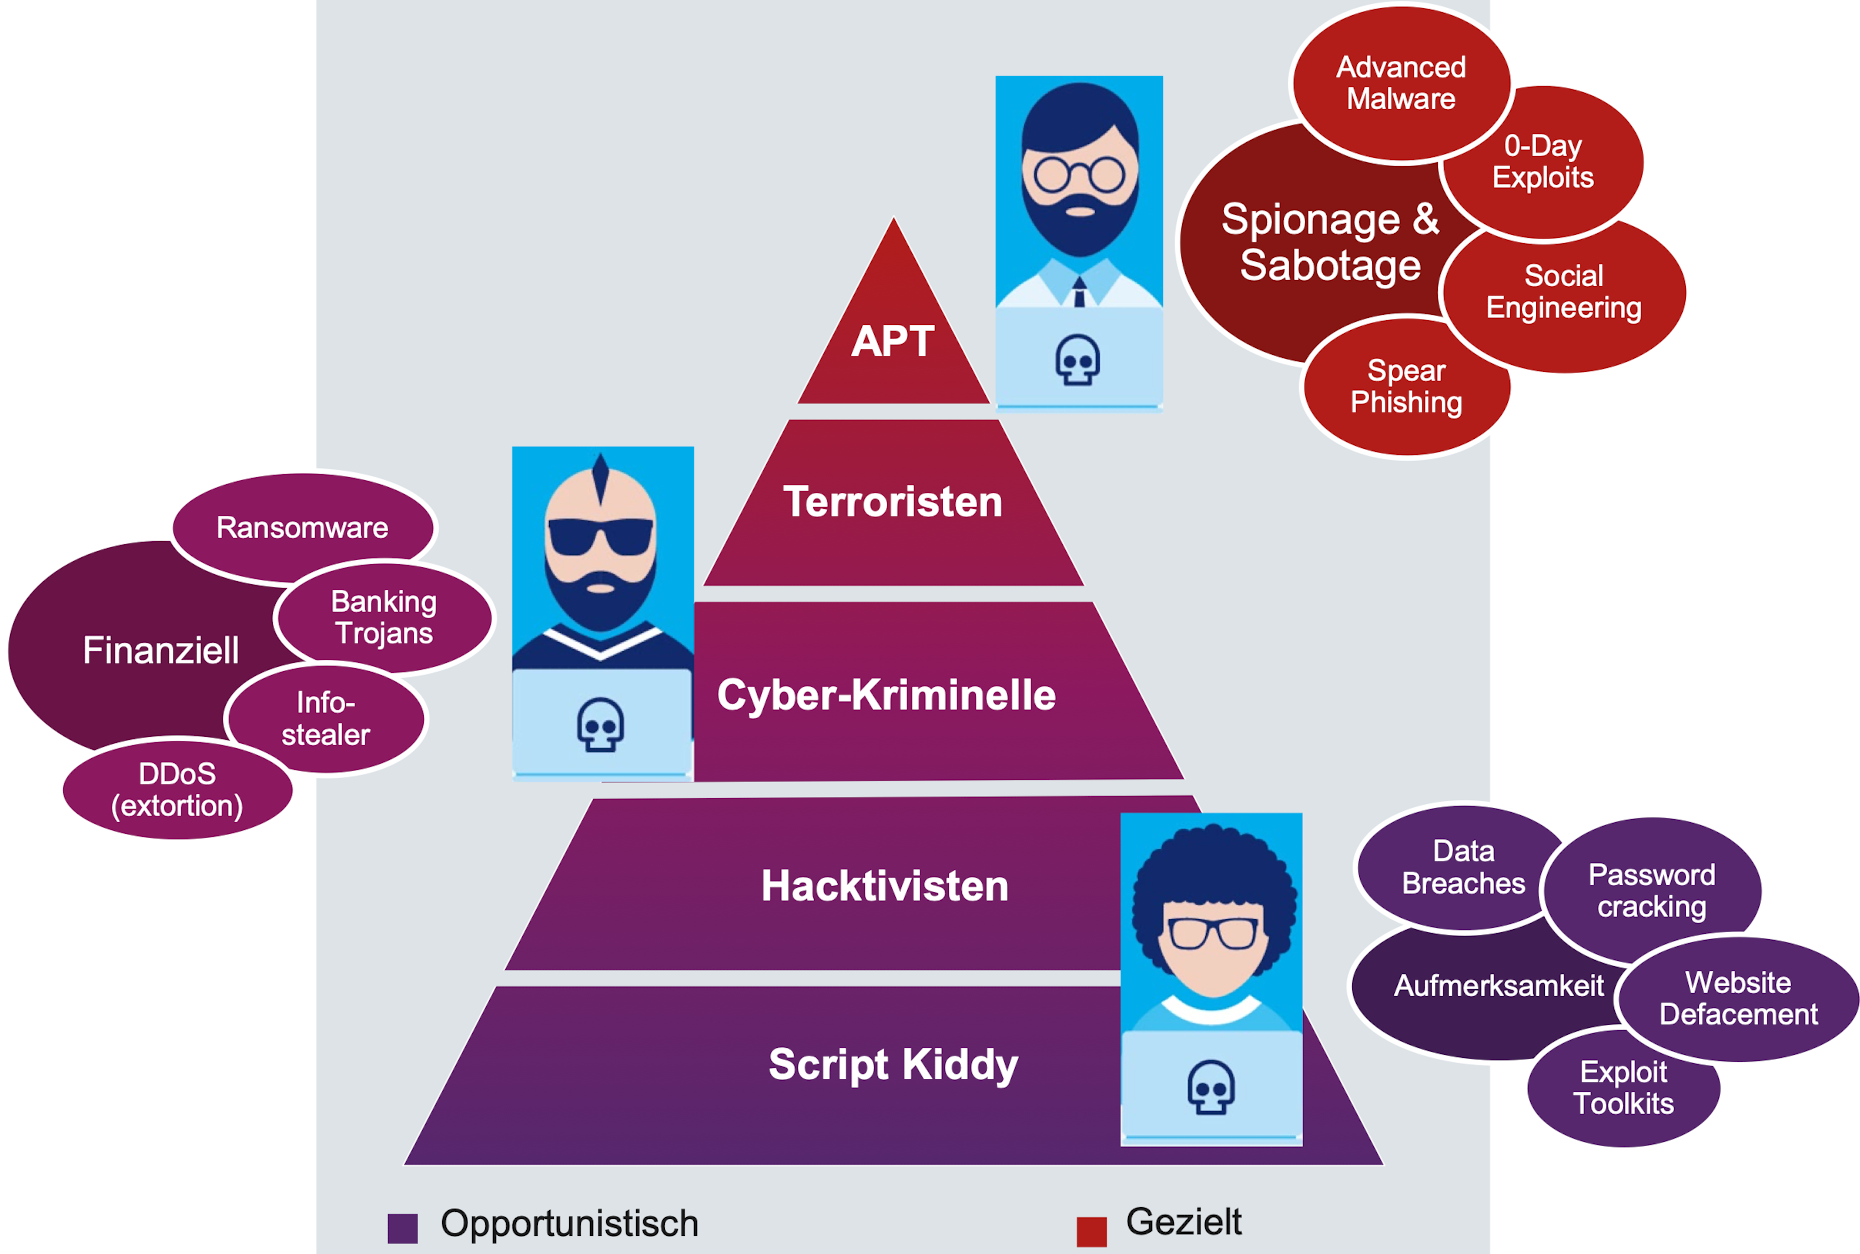
\includegraphics[width=.8\linewidth]{./img/01-cyber_defense/threat_actors}
    \vspace{-8pt}
\end{center}


\subsection{Script Kiddy}
\vspace{-8pt}
\begin{multicols*}{2}
    \textbf{Motivation}
    \begin{itemize}
        \item Aufmerksamkeit
        \item Anerkennung unter Ihresgleichen
        \item Opportunistisch
    \end{itemize}
    \textbf{Fähigkeiten}
    \begin{itemize}
        \item Wenige Fähigkeiten und Kenntnisse
        \item Nutzen verfügbare Hacking Tools
    \end{itemize}
\end{multicols*}
\vspace{-8pt}


\subsection{Hacktivisten}
\vspace{-8pt}
\begin{multicols*}{2}
    \textbf{Motivation}
    \begin{itemize}
        \item Aufmerksamkeit
        \item Anerkennung unter Gleichgesinnten
        \item Protest zum Ausdruck bringen
        \item Gezielt
    \end{itemize}
    \textbf{Fähigkeiten}
    \begin{itemize}
        \item Variieren sehr stark
        \item Wenig bis sehr Fortgeschritten
    \end{itemize}
\end{multicols*}
\vspace{-8pt}


\subsection{Übersicht: Script Kiddy \& Hacktivisten}
\begin{minipage}{0.3\linewidth}
    \begin{itemize}
        \item \textbf{P0:}\\ Erster eingenommener Server
        \item \textbf{TD:}\\ Ziel des Angreifers
    \end{itemize}
\end{minipage}
\begin{minipage}{0.7\linewidth}
    \begin{center}
        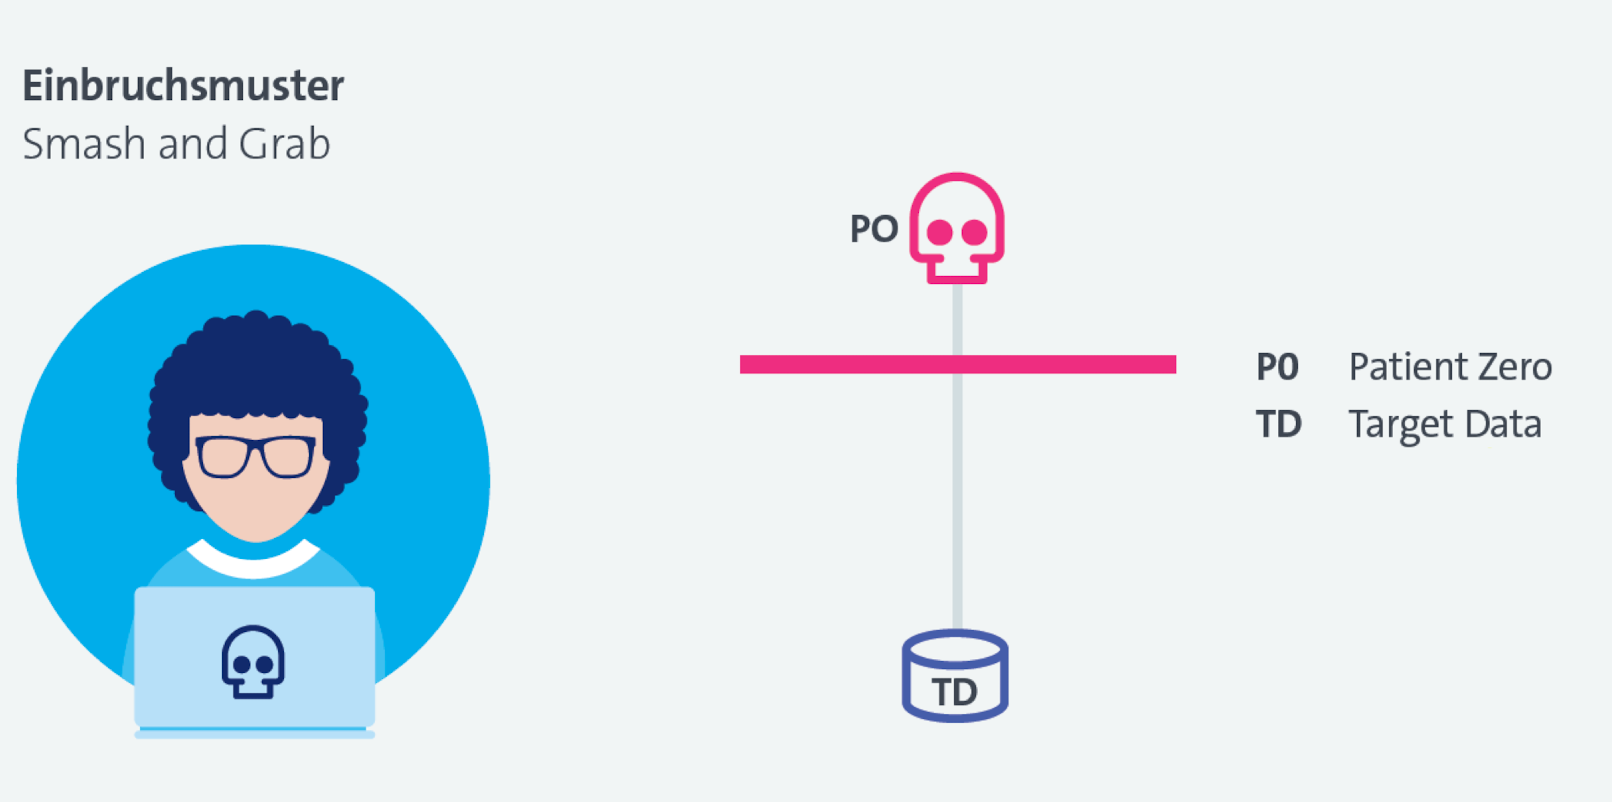
\includegraphics[width=\linewidth]{./img/01-cyber_defense/script_hacktivist}
    \end{center}
\end{minipage}

\textbf{Script Kiddys} und \textbf{Hacktivisten} zielen primär auf direkt exponierte Systeme ab wie beispielsweise Webserver. Sie zeichnen sich dadurch aus, dass sie schnellstmöglich ihren «Smash and Grab-Erfolg» bekannt geben wollen. Sie dringen in den wenigsten Fällen über längere Zeit in Netzwerke ein.


\subsection{Cyber-Kriminelle}
\vspace{-8pt}
\begin{multicols*}{2}
    \textbf{Motivation}
    \begin{itemize}
        \item Finanzieller Art, erpressen sehr viel Geld oder stehlen wertvolle Daten
        \item Opportunistisch
    \end{itemize}
    \textbf{Fähigkeiten}
    \begin{itemize}
        \item Hohe Professionalisierung
        \item Insider bieten in Untergrundforen an
        \item Setzen Angriffsmittel gegen eine breite Palette von Zielen ein
    \end{itemize}
\end{multicols*}

\subsection{Terroristen}
\vspace{-8pt}
\begin{multicols*}{2}
    \textbf{Motivation}
    \begin{itemize}
        \item Sabotage, Schaden \& Chaos anrichten
        \item Angst verbreiten
        \item Aufmerksamkeit und Rekrutierung
    \end{itemize}
    \textbf{Fähigkeiten}
    \begin{itemize}
        \item Angriffe auf kritische Systeme befürchtet, aber noch keine bekannt
        \item Nicht-staatliche, terroristische Gruppen scheinen Fähigkeit für gezielte Cyber-Angriffe noch nicht aufgebaut zu haben
    \end{itemize}
\end{multicols*}
\vspace{-8pt}


\subsection{Übersicht: Cyber-Kriminelle \& Terroristen}
\begin{minipage}{0.3\linewidth}
    \begin{itemize}
        \item \textbf{P0:}\\ Erster eingenommener Server
        \item \textbf{TD:}\\ Ziel des Angreifers
        \item \textbf{LM:}\\ Bewegung im\\ Netzwerk
        \item \textbf{P:}\\ Hintertüre
    \end{itemize}
\end{minipage}
\begin{minipage}{0.7\linewidth}
    \begin{center}
        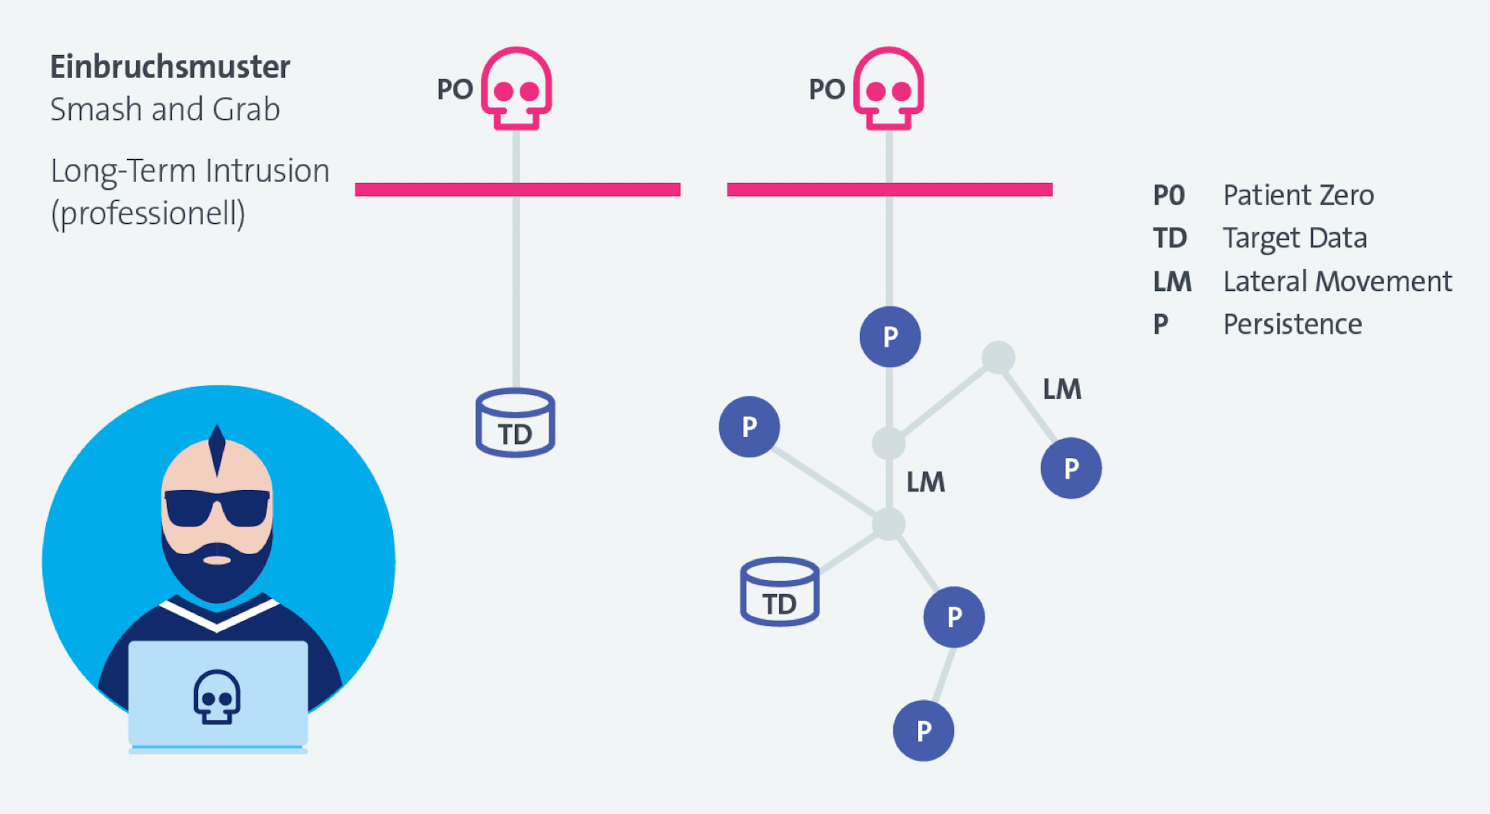
\includegraphics[width=\linewidth]{./img/01-cyber_defense/cyber_terrorists}
    \end{center}
\end{minipage}

\textbf{Cyber-Kriminelle} benötigen eine erheblich lange Verweildauer in den Systemen, um an die gewünschten Daten zu kommen und stehen oftmals in ihren technischen Fähigkeiten vielen APTs in nichts nach. Der entscheidende
Unterschied liegt jedoch in den strategischen Zielen.